\subsubsection{Clasificador de cultivos}

El sistema de clasificación determina la presencia o ausencia de lechuga en una posición de cultivo y su estado de madurez. Se implementó mediante un algoritmo de clasificación morfológica basado en reglas explícitas derivadas del análisis estadístico de descriptores geométricos. A diferencia de métodos de aprendizaje profundo, este enfoque emplea segmentación cromática en espacio HSV seguida de clasificación por umbrales sobre el descriptor de área del contorno principal detectado. Este clasificador discrimina entre lechugas maduras y no maduras (plantines/vasos vacíos), proporcionando precisión adecuada con costo computacional reducido compatible con ejecución en tiempo real.\\

Etapa 1: Segmentación cromática\\
\noindent
El sistema explota el contraste cromático entre las lechugas verdes y el entorno del sistema hidropónico (tubos blancos de PVC). La segmentación se realiza definiendo un rango de valores en los tres canales del espacio HSV correspondiente a las tonalidades verdes de las lechugas hidropónicas.

Cada píxel se evalúa individualmente: si sus componentes de matiz, saturación y valor se encuentran dentro de los límites establecidos, se marca como vegetación. Esta operación genera una máscara binaria donde las regiones blancas corresponden a vegetación detectada y las regiones negras al resto de la escena.

\begin{figure}[H]
\centering
\begin{subfigure}[b]{0.45\textwidth}
    \centering
    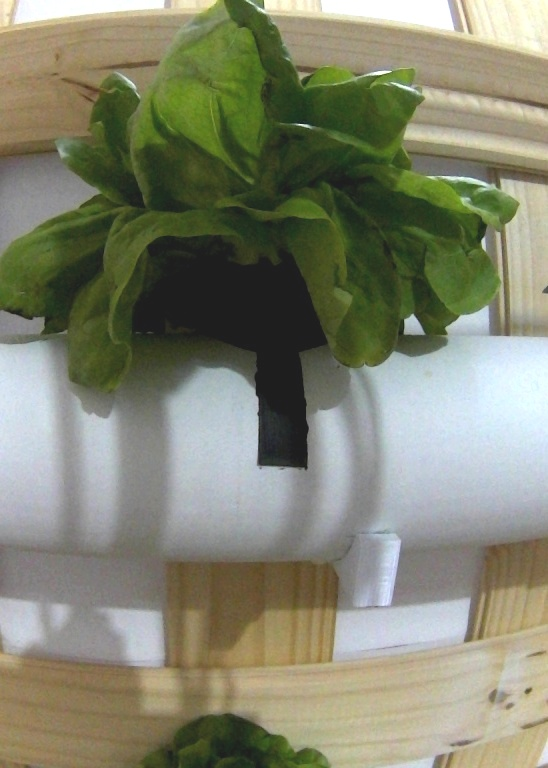
\includegraphics[width=0.6\textwidth]{imagenes/clasificador_1_original.jpg}
    \caption{Imagen RGB original}
\end{subfigure}
\hfill
\begin{subfigure}[b]{0.45\textwidth}
    \centering
    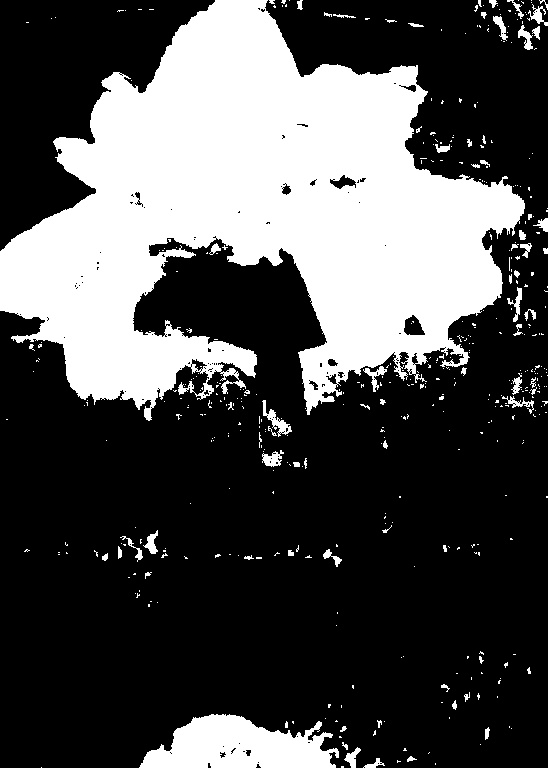
\includegraphics[width=0.6\textwidth]{imagenes/clasificador_2_verde.jpg}
    \caption{Máscara de vegetación verde}
\end{subfigure}
\caption{\textit{Etapa 1: Segmentación cromática en espacio HSV}}
\label{fig:clasificador_etapa1}
\end{figure}

Etapa 2: Refinamiento morfológico\\
\noindent
La máscara binaria presenta imperfecciones causadas por variaciones locales de iluminación y limitaciones del sensor. Se aplica una secuencia de operaciones morfológicas para refinarla:

\begin{itemize}[label=$\bullet$]
    \item \underline{Cierre morfológico}: Rellena huecos pequeños dentro de las regiones y conecta componentes próximos fragmentados.
    \item \underline{Apertura morfológica}: Elimina píxeles aislados y pequeñas protuberancias correspondientes a ruido.
\end{itemize}

Aplicación de kernels de convolución.\\
\noindent
Las operaciones morfológicas mencionadas se implementan mediante convolución con elementos estructurantes (kernels) específicos descriptos en la sección 2.2.1.\\ %La secuencia completa de refinamiento aplica los siguientes kernels iterativamente:

%\begin{table}[H]
%\centering
%\label{tab:kernels_clasificador}
%\begin{tabular}{|l|c|l|p{5.5cm}|}
%\hline
%\textbf{Kernel} & \textbf{Dimensiones} & \textbf{Operaciones} & \textbf{Propósito} \\ \hline
%\texttt{kernel\_small} & 3×3 & OPEN, CLOSE & Limpieza básica de máscaras (2 iter.) \\ \hline
%\texttt{kernel\_medium} & 5×5 & CLOSE & Conectar regiones próximas (2 iter.) \\ \hline
%\texttt{kernel\_vertical} & 7×3 & CLOSE & Conectividad vertical preferencial (1 iter.) \\ \hline
%\texttt{kernel\_edge} & 2×2 & DILATE & Engrosar bordes Canny (1 iter.) \\ \hline
%\texttt{kernel\_auxiliar} & 5×3 & CLOSE & Extensión vertical de regiones negras \\ \hline
%\end{tabular}
%\caption{Kernels utilizados en el refinamiento morfológico del clasificador}
%\end{table}
Cada kernel se aplica mediante convolución según la ecuación 2.2, donde el elemento estructurante $B$ define la forma y alcance del vecindario considerado. En todos los casos el kernel es una matriz (\textbf{B}) de unos en su diagonal y la matriz \textbf{A} proviene de la aplicación de algun filtro anterior a la operación morfologica. La secuencia típica de aplicación es:%Por ejemplo:

%\begin{itemize}[label=$\bullet$]
%    \item \textbf{kernel\_small (3×3)}: Elemento cuadrado isotrópico que afecta los 8 vecinos inmediatos del píxel central. Se emplea como compromiso entre eliminación de ruido y preservación de detalles relevantes.
    
%    \item \textbf{kernel\_medium (5×5)}: Elemento con mayor alcance espacial (24 píxeles alrededor) utilizado para cerrar huecos más grandes y conectar componentes fragmentados por variaciones de iluminación.
    
%    \item \textbf{kernel\_vertical (7×3)}: Elemento estructurante rectangular con preferencia vertical (mayor alcance en eje Y). Diseñado específicamente para unificar regiones de lechugas que aparecen fragmentadas verticalmente debido a variaciones cromáticas entre hojas superiores e inferiores.
    
%    \item \textbf{kernel\_edge (2×2)}: Elemento pequeño para dilatación controlada de bordes detectados por Canny, ampliando ligeramente su grosor sin conectar estructuras distantes.
%\end{itemize}

\begin{enumerate}
    \item Se realiza una operación morfológica de apertura (ec. \ref{eq:apertura_morf}) con \texttt{kernel (3x3, 2 iter.)} donde se elimina ruido puntual. %A es la imagen obtenida luego de la aplicación del filtro de saturación y B el kernel.
    \item Se realiza una operación morfológica cierre (ec. \ref{eq:cierre_morf}) con \texttt{kernel (3x3, 2 iter.)} donde se rellena huecos pequeños.  
    \item Se realiza una operación morfológica cierre (ec. \ref{eq:cierre_morf}) con \texttt{kernel (5x5, 1 iter.)} donde se conecta regiones próximas.
    \item Se realiza una operación morfológica cierre (ec. \ref{eq:cierre_morf}) con \texttt{kernel (7x3, 1 iter.)} donde se unifica fragmentos verticales.
    \item Se realiza una operación morfologica de dilatación (ec \ref{eq:dilatacion_morf}) con \texttt{kernel (2x2, 1 iter.)} donde se engrosan los bordes detectados por Canny.
\end{enumerate}

%El número de iteraciones fue determinado empíricamente mediante evaluación visual sobre el conjunto de calibración (80\% del dataset), seleccionando la configuración que maximizaba la continuidad de las regiones de vegetación sin introducir conexiones espurias con elementos del fondo.

%Se emplea un elemento estructurante rectangular de 3×3 píxeles como compromiso entre eliminación de ruido y preservación de detalles relevantes.

\begin{figure}[H]
\centering
\begin{subfigure}[b]{0.48\textwidth}
    \centering
    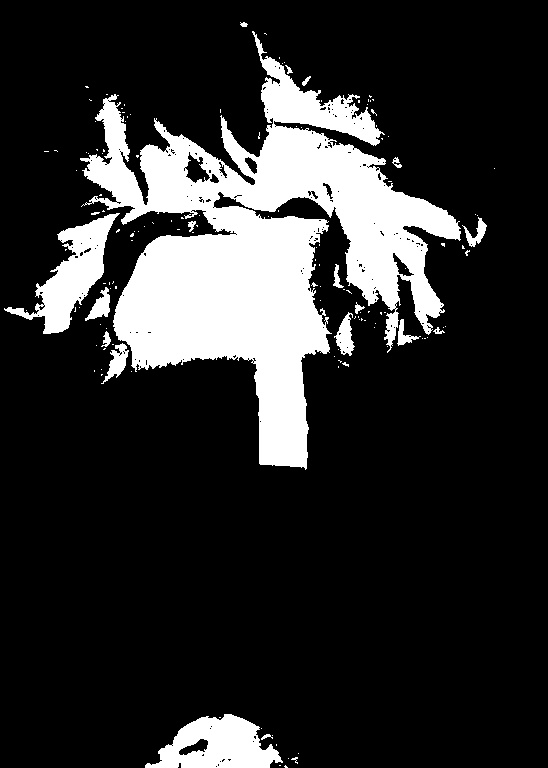
\includegraphics[width=0.6\textwidth]{imagenes/clasificador_3_negro.jpg}
    \caption{Máscara de regiones oscuras}
\end{subfigure}
\hfill
\begin{subfigure}[b]{0.48\textwidth}
    \centering
    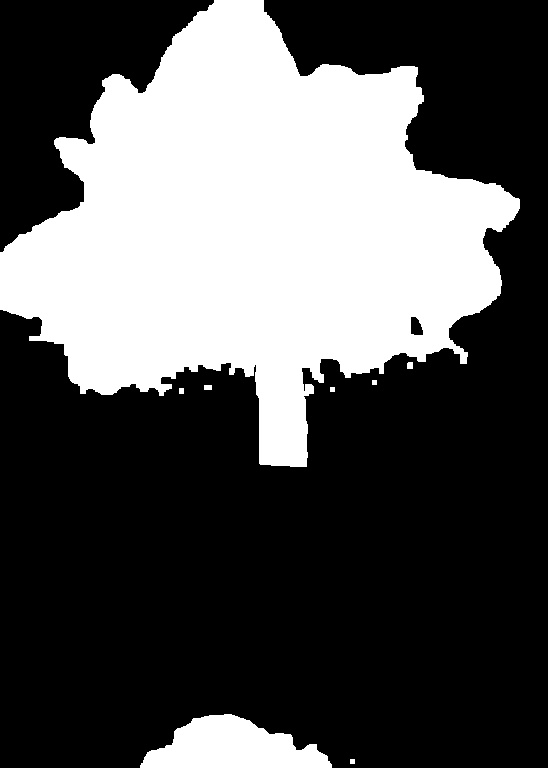
\includegraphics[width=0.6\textwidth]{imagenes/clasificador_4_combinado.jpg}
    \caption{Combinación verde + negro}
\end{subfigure}

\vspace{0.3cm}

\begin{subfigure}[b]{0.48\textwidth}
    \centering
    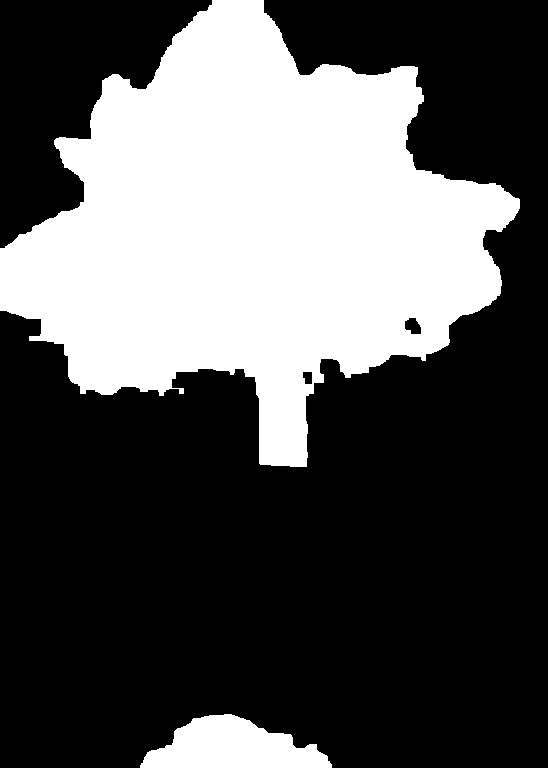
\includegraphics[width=0.6\textwidth]{imagenes/clasificador_5_binario_final.jpg}
    \caption{Máscara binaria refinada}
\end{subfigure}
\hfill
\begin{subfigure}[b]{0.48\textwidth}
    \centering
    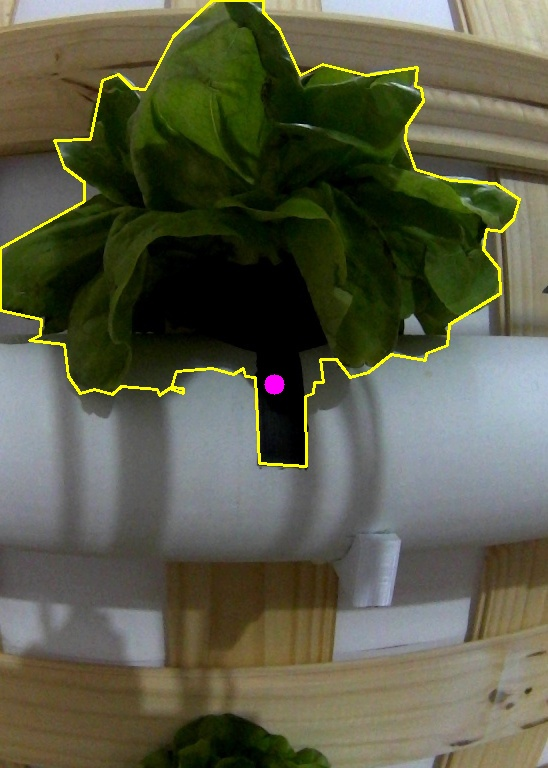
\includegraphics[width=0.6\textwidth]{imagenes/clasificador_6_contornos.jpg}
    \caption{Contornos finales detectados}
\end{subfigure}

\caption{\textit{Etapas del algoritmo de clasificación morfológica}}
\label{fig:clasificador_etapa2}
\end{figure}

Etapa 3: Detección y filtrado de contornos\\
\noindent
Sobre la máscara refinada se ejecuta detección de contornos que identifica las fronteras entre vegetación y fondo. Se emplea extracción de contornos externos únicamente, dado que las lechugas no presentan huecos internos relevantes.

Los contornos detectados se filtran por área mínima de 5000 píxeles, eliminando ruido residual y pequeñas sombras. De los contornos válidos, se selecciona el de mayor área bajo la hipótesis de que la lechuga constituye el objeto verde dominante en la escena.\\

Etapa 4: Clasificación por área\\
\noindent
El área del contorno seleccionado (en píxeles) constituye el descriptor empleado para clasificación. Se compara contra umbrales establecidos estadísticamente mediante análisis de muestras representativas. Áreas superiores al umbral indican lechuga madura lista para cosecha, mientras que áreas inferiores corresponden a plantas inmaduras o posiciones vacías.\\
Cuando no se detectan contornos válidos, el sistema clasifica la posición como vacía con alta confianza.
\subsubsection{Métricas de desempeño}
Evaluado sobre 25 imágenes de validación independientes:

\begin{table}[H]
\centering
\begin{tabular}{|l|c|c|c|c|}
\hline
\textbf{Clase} & \textbf{Precisión} & \textbf{Recall} & \textbf{F1-Score} & \textbf{Muestras} \\ \hline
Lechuga madura & 90.0\% & 90.0\% & 0.90 & 10 \\ \hline
Plantín/inmadura & 77.8\% & 87.5\% & 0.82 & 8 \\ \hline
Vaso vacío & 100\% & 85.7\% & 0.92 & 7 \\ \hline
\textbf{Promedio ponderado} & \textbf{88.2\%} & \textbf{88.0\%} & \textbf{0.88} & \textbf{25} \\ \hline
\end{tabular}
\caption{Métricas por clase del clasificador de lechugas}
\label{tab:metricas_lechugas}
\end{table}

Matriz de confusión del clasificador de lechugas:

\begin{table}[H]
\centering
\begin{tabular}{cc|c|c|c|}
\cline{3-5}
& & \multicolumn{3}{c|}{\textbf{Predicción}} \\ \cline{3-5}
& & Madura & Inmadura & Vacío \\ \hline
\multicolumn{1}{|c|}{\multirow{3}{*}{\textbf{Real}}} & Madura & 9 & 1 & 0 \\ \cline{2-5}
\multicolumn{1}{|c|}{} & Inmadura & 1 & 7 & 0 \\ \cline{2-5}
\multicolumn{1}{|c|}{} & Vacío & 0 & 0 & 7 \\ \hline
\end{tabular}
\caption{Matriz de confusión multiclase - lechugas}
\label{tab:confusion_lechugas}
\end{table}

\noindent
Análisis de errores:
\begin{itemize}
        \item Confusión madura $\leftrightarrow$ inmadura (2 casos): plantas en estado de transición con área $\approx$18,000 px cercana al umbral de decisión
    \end{itemize}


Validación de repetibilidad\\
\noindent
Para evaluar la consistencia, se realizaron 10 capturas consecutivas de la misma escena:

\begin{table}[H]
\centering
\begin{tabular}{|l|c|c|}
\hline
\textbf{Detector} & \textbf{Consistencia} & \textbf{Varianza espacial} \\ \hline
Cintas & 100\% (10/10) & $\sigma_x = 0.8$ px, $\sigma_y = 1.2$ px \\ \hline
Tubos & 100\% (10/10) & $\sigma_y = 2.1$ px \\ \hline
Lechugas & 90\% (9/10) & N/A (categórico) \\ \hline
\end{tabular}
\caption{Repetibilidad de detectores}
\label{tab:repetibilidad}
\end{table}

\noindent
La variación en el clasificador de lechugas ocurrió en una muestra con área fluctuando entre 18,200-18,800 px debido a variaciones de iluminación, confirmando la necesidad de zona de incertidumbre alrededor de umbrales.

%Tiempos de procesamiento.\\
%\noindent
%Medidos en Raspberry Pi 5 (procesador ARM Cortex-A76 quad-core a 2.4 GHz):

%\begin{table}[H]
%\centering
%\begin{tabular}{|l|c|c|}
%\hline
%\textbf{Detector} & \textbf{Tiempo medio} & \textbf{Desviación estándar} \\ \hline
%Cintas & 32 ms & 4 ms \\ \hline
%Tubos & 48 ms & 7 ms \\ \hline
%Lechugas & 41 ms & 5 ms \\ \hline
%\end{tabular}
%\caption{Tiempos de procesamiento por detector}
%\label{tab:tiempos_procesamiento}
%\end{table}